% Ray tracing structures on the GPU has been mapped more or less 100%
% from CPU structures. We need to build them for the GPU instead. That
% means rethinking some of the algorithms (like add persistent
% threads.)



\chapter{Ray Tracing}\label{chp:rayTracing}

\chapterquote{Some argue that in the very long term, rendering may best be
  solved by some variant of ray tracing, in which huge numbers of rays sample
  the environment for the eye’s view of each frame. And there will also be
  colonies on Mars, underwater cities, and personal jet packs.}{Tomas Möller and
  Eric Haines}


% Motivate!

% An optimized ray tracer will be used to test whether or not more time
% spent on creating a better kD tree will pay off in final rendering
% time.

In this chapter we shall look at how to implement a ray tracer and how it can be
optimized to run efficiently on GPUs using NVIDIA's CUDA framework. The result
will be an optimized ray tracer, which will be used in \refchapter{chp:results}
to evaluate the quality of kd-trees.

A ray, $r$, is defined as a line which starts at a point called \textit{origin},
$r_{ori}$, and can be traced infinitely along a certain \textit{direction},
$r_{dir}$. Using $t$ to describe the distance traveled along the ray, $r$ can
then be described as $r(t) = t \cdot r_{dir} + r_{ori}$. Tracing a ray into the
scene to find the nearest intersecting triangle, then means finding the triangle
that the ray intersects at the lowest value of $t$. Before the actual ray
tracing can be performed, the primary rays traced from the camera and into the
scene must be computed and stored as a list of rays, $rays$. How these rays are
generated is a large topic in itself and lies outside the scope of this
thesis. Chapter 6 in \citebook{PBR:2010} provides good insight into the theory
needed for creating the primary rays.

The general structure for a ray tracer that handles reflective surfaces can be
seen in \refalg{alg:generalRayTracer}. \Refalg{alg:generalRayTracer} takes as
input a list of rays to be traced, $rays$, the scene that should be ray traced,
$scene$, and the image, $pixels$, on which the ray traced scene should be
drawn. Each ray is independent of the other rays and can therefore be traced in
parallel by the GPU. The algorithm first determines which of the triangles
intersected by the ray is closest to the ray's origin, i.e. the triangle first
\textit{seen} by the ray. It then computes the color of the triangle intersected
by the ray and blends that color with the color that has been accumulated so far
in $pixels[r]$. How the color is computed is not relevant to the kd-tree
evaluations in \refchapter{chp:results} and is therefore not discussed in this
thesis. Suffice it to say that the ray tracer produced as part of the thesis
uses the \textit{general lighting equation} described on page 83 in
\citebook{RTR2}. Finally the algorithm checks if a triangle is reflective and if
so then a reflection ray is generated and added to the $nextRays$ list. A
reflection ray's direction, $ref_{dir}$ is calculated from the triangle's
normal, $n$, and the incoming rays direction, $ray_{dir}$

\begin{displaymath}
  ref_{dir} = -2 (n \cdot ray_{dir}) n + ray_{dir}
\end{displaymath}

The new origin of the reflection ray is simply the intersection point of the
incoming ray and the triangle. As long as one or more reflection rays are
generated by the traced rays, the ray tracing process is repeated.

\begin{algorithm}
  \caption{A general ray tracer.}
  \label{alg:generalRayTracer}
  \begin{algorithmic}
    \PROCEDURE{RayTracer}
              {$rays$ : Ray List, $scene$ : Scene Description, $pixels$ : Image}
              {$pixels$ : Image}{
                \PARALLELFOR{$r$}{$rays$}
                  \COMMENTIT{The scene description can be either a list of
                    triangles in the scene, or a kd-tree created from those
                    triangles.}
                  \ASSIGN{$triangle$}{ClosestIntersectingTriangle$(r, scene)$}
                  \ASSIGN{$pixels[r]$}{ComputeColor$(pixels[r], r, triangle)$}
                  \DECLARE{$nextRays$}{Ray List}
                  \IF{IsReflective$(triangle)$}
                    \STATE{$nextRays$.Add(GenerateReflectionRay$(triangle, ray)$)}
                  \ENDIF
                \ENDFOR
                \IF{$nextRays$.NotEmpty}
                  \ASSIGN{$pixels$}{RayTracer$(nextRays, scene, pixels)$}
                \ENDIF
              }
  \end{algorithmic}
\end{algorithm}

In this chapter I will present two methods for determining which triangle in a
scene a ray intersects. In \refsection{sec:exhaustive} I present an exhaustive
ray tracer, which finds the closest intersection point by intersecting each ray
with every triangle. In \refsection{sec:hierarchicalTraversal} I then present a
hierarchical ray tracer, which will use the kd-tree to minimize the number of
triangles each ray needs to be intersected with. In the same section I will
describe three optimizations that can be applied to hierachical ray tracers
running on GPUs. The optimizations will be added incrementally to the
hierarchical ray tracer and implementation details to each specific optimization
is therefore discussed alongside the theory. The optimized ray tracer will use
the \textit{short-stack} optimization from \horn, a \textit{packet scheme}
inspired by Wald et al.\citebook{Wald:2001:IRCRT} and an optimization inspired
by Empty Space Maximization, that utilizes a leaf node's bounding box, which is
computed while creating the kd-tree.

In \refsection{sec:exhaustive} and \refsection{sec:hierarchicalTraversal} I will
merely have assumed that a method exists for determining if and where a ray and
a triangle intersects. In the final section of this chapter I will discuss two
such methods with respect to the GPU's memory hierarchy and maximizing
occupancy.

The ray tracers and their optimization will be evaluated in
\refchapter{chp:results} and hopefully show that the hierarchical ray tracer is
faster than the exhaustive ray tracer. This will be a very important result, as
the time spent rebuilding acceleration structures for dynamic scenes would
otherwise be wasted.




\section{Exhaustive Ray Tracing} \label{sec:exhaustive}

Before directing our focus on hierarchical ray tracers, we will first
take a look at an exhaustive ray tracer.

% GPU does bruteforcing well.

The reason that an exhaustive ray tracer is interesting is that the GPU comes
with high computational power, but little tolerance for branching, as was
discussed in \refsection{sec:threadHierarchy}. An exhaustive ray tracer fits
very well onto such an architecture, since intersecting each ray with every
triangle certainly requires a lot of computational power, and every ray in a
warp will loop over the same triangles and therefore not branch independently.

%, so the triangle-loop will not cause thread divergence.

% Algorithm

The ClosestIntersectingTriangle procedure used by \refalg{alg:generalRayTracer}
is implemented in \refalg{alg:exhaustive} using an exhaustive ray tracer. The
actual ray tracers implemented in this thesis also compute and return a ray's
barycentric coordinates on the triangle it intersects, which is explained in
\refsection{sec:intersection}. The barycentric coordinates are used to perform
lighting calculations, but in order to keep the algorithms simple and
instructive, this has been omitted and is assumed to be performed by the
ComputeColor method invoked in \refalg{alg:generalRayTracer}.


\begin{algorithm}
  \caption{An exhaustive implementation of ClosestIntersectingTriangle}
  \label{alg:exhaustive}
  \begin{algorithmic}
    \PROCEDURE{ClosestIntersectingTriangle}
              {$R$ : Ray, $Ts$, Triangle List}
              {$t_{near}$ : Triangle}{
                \ASSIGN{$t_{near}$}{$NULL$}
                \FOREACH{$t$}{$Ts$}
                  \ASSIGN{$t_{near}$}{ClosestHit$(t, t_{near})$}
                \ENDFOR
              }
  \end{algorithmic}
\end{algorithm}

The downside to the exhaustive approach is that intersecting a ray with $m$
triangles, yields a time complexity of $O(m)$.

\section{Hierarchical Ray Tracing}\label{sec:hierarchicalTraversal}

% Time complexity of O(n log m)

Hierarchical ray tracers provide a better upper bound than exhaustive ray
tracers. Given a hierachical data structure over $m$ geometric primitives in a
scene, the leaf node that a ray should traverse next can be found in $O(\log m)$
time. This is significantly better than the exhaustive ray tracer from
\refsection{sec:exhaustive}.

% Describe how the tree is traversed

When ray tracing a scene using a kd-tree as acceleration structure, each ray
traverses the tree in search of the leaf node closest to the rays origin, while
still being in front of the ray. The leaf nodes is hereafter refered to as the
\textit{nearest leaf}. At each interior node, the ray needs to determine which
of the child nodes it should traverse next. This process is continued until a
leaf node is reached. The ray then needs to intersect each triangle in the leaf
and determine which intersected triangle is nearest, if any. If the ray
intersects a triangle, then it reports this intersection, otherwise it needs to
continue traversing the tree. How this is done is the topic of
\refsection{sec:kdRestart} and \refsection{sec:shortStack}. The general
algorithm for ray tracing a kd-tree can be seen in \refalg{alg:generalTracing}.

\begin{algorithm}
  \caption{A general kd-tree traversal algorithm for ray tracing}
  \label{alg:generalTracing}
  \begin{algorithmic}
    \PROCEDURE{ClostestIntersectingTriangle}
              {$ray$ : Ray, $tree$ : kd-tree}
              {$t_{near}$ : Triangle}{
                \ASSIGN{$t_{near}$}{$NULL$}
                \WHILE{ray inside scene}
                  \COMMENTIT{Traverse the tree until the leaf node nearest the
                    ray origin is found and store the distance to the nearest
                    splitting plane the ray intersects in $d_{split}$.}
                  \ASSIGN{$(leaf, d_{split})$}{TraverseTree($ray, tree$)}
                  \COMMENTIT{Intersect triangles in leaf and return the nearest
                    intersected triangle, if any.}
                  \ASSIGN{$t_{near}$}{Intersect($ray, leaf.triangles$)}
                  \COMMENTIT{Break if a closest intersection
                    is found and return it.}
                  \IF{$t_{near} \neq NULL$}
                    \STATE{\textbf{break}}
                  \ELSE
                    \ASSIGN{$ray.origin$}{$ray.origin + d_{split} * ray.direction$}
                  \ENDIF
                \ENDWHILE
              }
  \end{algorithmic}
\end{algorithm}

% Traversal method

The method used to determine which of an interior node's children to visit next
can be seen in \refalg{alg:generalTraversal}. For each interior node the ray
first needs to determine which of the two children are placed \textit{nearest}
and \textit{farthest} along the rays direction. It then computes the signed
distance from the ray to the nodes splitting plane. If this distance is below 0
then the plane is located behind the ray and the farthest child must be
visited. If the distance is above 0 then the nearest node needs to be visited
next. In addition the distance, $d_{split}$, to the nearest splitting plane in
front of the ray needs to be updated. $d_{split}$ is used to advance the ray
beyond a visited leaf node if it did not intersect any geometry.

\begin{algorithm}
  \caption{A basic kd-tree traversal algorithm}
  \label{alg:generalTraversal}
  \begin{algorithmic}
    \PROCEDURE{TraverseTree}
              {$ray$ : Ray, $tree$ : kd-tree}
              {$leaf$ : Node, $d_{split}$ : Number}{
                \ASSIGN{$d_{split}$}{$\infty$}
                \ASSIGN{$node$}{$tree.root$}
                \WHILE{$node \neq LEAF$}
                  \COMMENTIT{The signed distance to the nodes splitting plane.}
                  \ASSIGN{$node_{near}$}{$ray.direction[node.axis] > 0$ ? $node.left$ : $node.right$}
                  \ASSIGN{$node_{far}$}{$ray.direction[node.axis] > 0$ ? $node.right$ : $node.left$}
                  \ASSIGN{$d_{node}$}{($node.splitValue - ray.origin[node.axis]) / ray.direction[node.axis]$}
                  \IF{$0 < d_{split}$}
                    \ASSIGN{$node$}{$node_{near}$}
                    \ASSIGN{$d_{split}$}{min$(d_{split}, d_{node})$}
                  \ELSE
                    \ASSIGN{$node$}{$node_{far}$}
                  \ENDIF
                \ENDWHILE
              }
  \end{algorithmic}
\end{algorithm}

In \reffig{fig:simpleScene} a simple scene consisting of four triangles is
shown. The corrosponding kd-tree matching the axis aligned splitting planes is
shown in \reffig{fig:simpleTree}. A tree traversal of the ray, $r(t) = t
\vectwoT{2}{1} + \vectwoT{0}{1}$, entering the scene in the lower left would
look like this: Upon entering the scene the ray first visits the root node,
0. Node 0 splits the scene along the x-axis at $x=4$ and the rays distance to
that plane is then $d_{split} = (4 - 0) / 2 = 2$. The ray therefore proceeds to
the childnode $2 > 0$ ? $1$ : $2 = 1$. The signed distance to node 1's splitting
plane is $d_{node} = (4 - 1) / 1 = 3$ and the ray proceeds to node $1 > 0$ ?
$3$ : $2 = 3$, where it finds no primitives to intersect. The ray is then
advanced beyond the nearest splitting plane by advancing it $d_{split}$ along
its direction. The new ray becomes $r'(t) = r(t) + d_{split} \cdot r_{dir} =
r(t) + 2 \vectwoT{2}{1} = t \vectwoT{2}{1} + \vectwoT{4}{3}$. Since the ray did
not intersect any geometry and has not advanced beyond the scene, the traversal
process is restarted for $r'(t)$.


\begin{figure}
  \centering
  \subfloat[A simple scene subdivided by a kd-tree.]{
    \begin{tikzpicture}[y=0.5cm, x=0.5cm,font=\sffamily]
      \drawNode{0,0}{8,0}{8,6}{0,6}

      % Tris
      \drawTri{0,6}{1,4}{2,5}
      \draw (1,5) node{0};
      \drawTri{4,6}{3,4}{2,5}
      \draw (3,5) node{1};
      \drawTri{4,2}{5,6}{6,4}
      \draw (5,4) node{2};
      \drawTri{8,0}{7,2}{6,1}
      \draw (7,1) node{3};

      % Splits
      \draw (4,0) -- (4,6);
      \draw (0,4) -- (4,4);
      \draw (2,4) -- (2,6);
      \draw (4,2) -- (8,2);

      % Ray
      \drawRay{0,1}{2,2}

      %axes
      \draw[->] (0,0) -- coordinate (x axis mid) (9,0);
      \draw[->] (0,0) -- coordinate (y axis mid) (0,7);
      %ticks
      \foreach \x in {0,2,...,9}
     		\draw (\x,1pt) -- (\x,-3pt)
			node[anchor=north] {\x};
    	\foreach \y in {0,2,...,7}
     		\draw (1pt,\y) -- (-3pt,\y) 
     			node[anchor=east] {\y}; 
    \end{tikzpicture}
    \label{fig:simpleScene}
  }
  \hspace{20pt}
  \subfloat[The kd-tree matching the scene. Nodes contain information
    about which axis have been divided and where. Leaf nodes contain a
    set of the triangles they overlap.]{
    \begin{tikzpicture}[y=0.5cm, x=.5cm,font=\sffamily,
        level/.style={sibling distance=40mm/#1}]
      \node [visitedNode] (0){$\begin{array}{c}0\\x:4\end{array}$}
        child {node [visitedNode] (1) {$\begin{array}{c}1\\y:4\end{array}$}
          child {node [visitedLeaf] (e) {$\begin{array}{c}3\\\emptyset\end{array}$}}
          child {node [node] (3) {$\begin{array}{c}4\\x:2\end{array}$}            
            child {node [leaf] (e) {$\begin{array}{c}7\\\{0\}\end{array}$}}
            child {node [leaf] (e) {$\begin{array}{c}8\\\{1\}\end{array}$}}
          }
        }
        child {node [node] (2) {$\begin{array}{c}2\\y:2\end{array}$}
            child {node [leaf] (e) {$\begin{array}{c}5\\\{2\}\end{array}$}}
            child {node [leaf] (e) {$\begin{array}{c}6\\\{3\}\end{array}$}}
        };
    \end{tikzpicture}
    \label{fig:simpleTree}
  }
  \caption[A simple scene and its kd-tree.]{}
  \label{fig:simpleSceneTree}
\end{figure}


\subsection{KD-restart}\label{sec:kdRestart}

% KD restart is the simplest and fastest.

The approach presented above, where kd-tree traversal is restarted at the root
node, is known as \textit{kd-restart} and is one of the simplest algorithms for
ray tracing kd-trees. The reason for the name is that if a ray does not
intersect any triangles in the nearest leaf node, then it advances past that
leaf node using $d_{split}$ and restarts traversal from the root of the tree.

% Instead of advancing the ray simply update tMin

The algorithm in its entirety is presented in \refalg{alg:KDRestart}. Instead of
advancing the ray by updating its origin, a signed distance, $d_{min}$, is used
to determine how far a ray has traveled.

\begin{algorithm}
  \caption{A kd-restart implementation of ClosestIntersectingTriangle}
  \label{alg:KDRestart}
  \begin{algorithmic}
    \PROCEDURE{ClosestIntersectingriangle}
              {$ray$ : Ray, $tree$ : kd-tree}
              {$t_{near}$ : Triangle}{
                \ASSIGN{$t_{near}$}{$NULL$}
                \ASSIGN{$d_{min}$}{$0$}
                \WHILE{$d_{min} < \infty$}
                  \ASSIGN{$d_{split}$}{$\infty$}
                  \ASSIGN{$node$}{$tree.root$}
                  \COMMENTIT{Traverse the tree until a leaf node is reached}
                  \WHILE{$node \neq LEAF$}
                    \ASSIGN{$d_{node}$}{($node.splitPosition - ray.origin[node.axis]) / ray.direction[node.axis]$}
                    \IF{$d_{min} < d_{node}$}
                      \ASSIGN{$node$}{$ray.direction[node.axis] > 0$ ? $node.left$ : $node.right$}
                      \ASSIGN{$d_{split}$}{min$(d_{split}, d_{node})$}
                    \ELSE
                      \ASSIGN{$node$}{$ray.direction[node.axis] > 0$ ? $node.right$ : $node.left$}
                    \ENDIF
                  \ENDWHILE
                  \COMMENTIT{Test intersection with the leafs primitives}
                  \ASSIGN{$t_{near}$}{Intersect($ray, leaf.triangles$)}
                  \IF{$t_{near} \neq NULL$}
                    \STATE{\textbf{break}}
                  \ELSE
                    \COMMENTIT{Advance the ray beyond the next splitting plane.}
                    \ASSIGN{$d_{min}$}{$d_{split}$}
                  \ENDIF
                \ENDWHILE
              }
  \end{algorithmic}
\end{algorithm}

\subsection{Short-stack}\label{sec:shortStack}

% Kd-Restart traverses many of the same nodes, because 

When a ray triggers a restart in kd-restart, it will almost always traverse many
of the same interior nodes as it did in its previous traversel. The reason for
this is that kd-trees will often store spatially local nodes as local nodes in
the tree. CPU ray tracers utilize this property by pushing the not-visited child
of an interior node onto a stack and then resuming from the first node on that
stack instead of restarting. This can save a lot of resources otherwise spent on
traversing the tree, since the ray will now skip interior nodes already visited
and resume closer to the next leaf node.

CUDA's memory model, however, is not flexible enough for this approach, which
requires either dynamically allocating more memory if the stack is filled or
pre-allocating a \textit{large enough} stack in local memory to handle any given
kd-tree. This would require quite large amounts of memory for huge scenes and
might even require too much memory for practical use on today's graphics
cards. The solution proposed by \horn{} was to use a \textit{short-stack}, a
fixed-size, circular stack of $N$ elements, and then revert to using kd-restart
if the stack underflows. The circular nature of the short-stack means that the
stack will favor nodes near the leafs and overwrite nodes traversed at the top
of the kd-tree. Since the nodes near the leafs are the ones with the highest
associated traversal cost, these are exactly the ones we would like to be able
to resume from in future traversals. In their research \horn{} found that a
short-stack approach only visited 3\% more nodes compared to the unlimited stack
in CPU approaches.

% Only push usefull 'forward' nodes to the stack.

Obviously all child nodes can not be pushed onto the short-stack, as that would
force the rays to visit the entire kd-tree. Therefore restrictions need to be
formulated as to which nodes should be pushed onto the short-stack. The first
restriction is not to push nodes located behind the ray, since the ray can never
intersect these. The second restriction is not to push nodes where the distance
to the splitting plane is greater than $d_{split}$, as these would never be
visited in a kd-restart traversal. The reasoning for this is that if a ray
advances beyond the splitting plane of one of its parent nodes, it effectively
means the ray should never visit that nodes nearest subtree again and therefore
no nodes from that subtree should be stored in the short-stack. An
implementation of kd-restart with the short-stack optimization is shown in
\refalg{alg:ShortStack}.

\begin{algorithm}
  \caption{A short-stack implementation of ClosestIntersectingTriangle}
  \label{alg:ShortStack}
  \begin{algorithmic}
    \PROCEDURE{ClosestIntersectingTriangle}
              {$ray$ : Ray, $tree$ : kd-tree}
              {$t_{near}$ : Triangle}{
    \ASSIGN{$t_{near}$}{$NULL$}
    \ASSIGN{$d_{min}$}{$0$}
    \WHILE{$d_{min} < \infty$}
      \IF{$stack$.IsEmpty}
        \ASSIGN{$node$}{$tree.root$}
        \ASSIGN{$d_{split}$}{$\infty$}
      \ELSE
        \ASSIGN{$(node, d_{split})$}{$stack$.Pop}
      \ENDIF
      \COMMENTIT{Traverse the tree until a leaf node is reached}
      \WHILE{$node \neq LEAF$}
        \ASSIGN{$d_{node}$}{($node.splitPosition - ray.origin[node.axis]) / ray.direction[node.axis]$}
        \IF{$d_{min} < d_{node}$}
          \ASSIGN{$node$}{$ray.direction[node.axis] > 0$ ? $node.left$ : $node.right$}
          \IF{$d_{node} < d_{split}$}
            \STATE{stack.push($upperChild, d_{split}$)}
          \ENDIF
          \ASSIGN{$d_{split}$}{min$(d_{split}, d_{node})$}
        \ELSE
          \ASSIGN{$node$}{$ray.direction[node.axis] > 0$ ? $node.right$ : $node.left$}
        \ENDIF
      \ENDWHILE
      \COMMENTIT{Test intersection with the leafs primitives}
      \ASSIGN{$t_{near}$}{Intersect($ray, leaf.triangles$)}
      \IF{$d_{min} < t_{split}$}
        \STATE{\textbf{break}}
      \ELSE
        \COMMENTIT{Advance the ray beyond the next splitting plane.}
        \ASSIGN{$d_{min}$}{$d_{next}$}
      \ENDIF
    \ENDWHILE
              }
  \end{algorithmic}
\end{algorithm}

% Example

Let us look at a simple example of how the short-stack will speedup
traversal. Using the scene in \reffig{fig:simpleSceneTree} again, we saw
previously that the ray, $R(t) = t \vectwoT{2}{1} + \vectwoT{0}{1}$, will
traverse nodes 0, 1, and 3. At node 0 the distance to the splitting plane was 2,
meaning the splitting plane is in front and the child not traversed should be
pushed to the short-stack. At node 1 the distance was 3, so the ray intersects
node 1's splitting plane after node 0's. Node 1's other child therefore does not
need to be pushed to the stack. The result of the first traversal can be seen on
\reffig{fig:shortStack1}.

So far the short-stack traversal and kd-restart traversal have both chosen the
exact same path through the tree. But where kd-restart would have had to restart
its traversal from the root node, the short-stack allows the ray to start the
second traversal from node 2 and proceed to leaf 5, where the ray intersects
triangle 2.

In this simple example having a short-stack only allows the ray to skip one node
at the cost of maintaining and using a short-stack, which will cause a
significant overhead. Consequently having a short-stack will probably not
provide any speedup in this small example. But imagine this simple tree as a
subtree in a much larger scene, with perhaps ten levels of nodes above it. Then
a short-stack implementation allows the ray to skip those first eleven nodes,
which can yield quite a performance improvement.

\begin{figure}
  \centering

  \subfloat[The short-stack algorithm's first traversal of the scene
    from \reffig{fig:simpleSceneTree}. When the ray traversed node 0
    it pushed node 2 onto the short-stack.]{
    \begin{tikzpicture}[y=0.5cm, x=.5cm,font=\sffamily,
        level/.style={sibling distance=40mm/#1}]
      \node [visitedNode] (0){$\begin{array}{c}0\\x:4\end{array}$}
        child {node [visitedNode] (1) {$\begin{array}{c}1\\y:4\end{array}$}
          child {node [visitedLeaf] (e) {$\begin{array}{c}3\\\emptyset\end{array}$}}
          child {node [node] (3) {$\begin{array}{c}4\\x:2\end{array}$}            
            child {node [leaf] (e) {$\begin{array}{c}7\\\{0\}\end{array}$}}
            child {node [leaf] (e) {$\begin{array}{c}8\\\{1\}\end{array}$}}
          }
        }
        child {node [node] (2) {$\begin{array}{c}2\\y:2\end{array}$}
            child {node [leaf] (e) {$\begin{array}{c}5\\\{2\}\end{array}$}}
            child {node [leaf] (e) {$\begin{array}{c}6\\\{3\}\end{array}$}}
        };
                        
      % Short-stack
      \draw (10,-4.5) -- (10,-7.5) -- (12,-7.5) -- (12,-4.5) -- (10,-4.5);
      \draw (10, -6.5) -- (12, -6.5);
      \draw (10, -5.5) -- (12, -5.5);
      \draw (11, -7) node{2};
      \draw (11, -6) node{-};
      \draw (11, -5) node{-};
      \draw[->,line width=1pt] (12.7,-7) -- (12.2,-7);
    \end{tikzpicture}
    \label{fig:shortStack1}
  }
  \\
  \subfloat[The short-stack algorithm's second traversal of the scene
    from \reffig{fig:simpleSceneTree}. Traversal is resumed from the first
    node on the stack, which is 2.]{
    \begin{tikzpicture}[y=0.5cm, x=.5cm,font=\sffamily,
        level/.style={sibling distance=40mm/#1}]
      \node [node] (0){$\begin{array}{c}0\\x:4\end{array}$}
        child {node [node] (1) {$\begin{array}{c}1\\y:4\end{array}$}
          child {node [leaf] (e) {$\begin{array}{c}3\\\emptyset\end{array}$}}
          child {node [node] (3) {$\begin{array}{c}4\\x:2\end{array}$}            
            child {node [leaf] (e) {$\begin{array}{c}7\\\{0\}\end{array}$}}
            child {node [leaf] (e) {$\begin{array}{c}8\\\{1\}\end{array}$}}
          }
        }
        child {node [visitedNode] (2) {$\begin{array}{c}2\\y:2\end{array}$}
            child {node [visitedLeaf] (e) {$\begin{array}{c}5\\\{2\}\end{array}$}}
            child {node [leaf] (e) {$\begin{array}{c}6\\\{3\}\end{array}$}}
        };
                        
      % Short-stack
      \draw (10,-4.5) -- (10,-7.5) -- (12,-7.5) -- (12,-4.5) -- (10,-4.5);
      \draw (10, -6.5) -- (12, -6.5);
      \draw (10, -5.5) -- (12, -5.5);
      \draw (11, -7) node{-};
      \draw (11, -6) node{-};
      \draw (11, -5) node{-};
    \end{tikzpicture}
    \label{fig:shortStack2}
  }
  \caption[Short-stack kd-tree traversal.]{}
\end{figure}


\subsection{Packets}

% Packets: 2x2 packets on the CPU for to take advantage of SIMD
% instructions (Wald), warp size packets on the GPU. While
% \citebook{1230129} implemented packets, they merely assumed it would
% yield a speedup and did not provide any results. Aila2009 is against
% packets as they in practice seem to make it slower.

Using some form of \textit{packets} to accelerate ray tracing is quite a
standard technique. Packets were introduced to CPU ray tracers by Wald et
al.\citebook{Wald:2001:IRCRT}, who utilized \textit{SIMD}\footnote{Single
  instruction, multiple data.} instructions to trace rays in packets of four
rays at a time. \horn{} extended their short-stack implementation with another
form of packet tracing, where individual threads would trace multiple rays to
amortize the cost of traversing the tree. Unfortunately tracing several rays in
one thread increases thread incoherence across threads in a warp and \aila{}
concludes that

\quotebook{It is worth noticing that [kd-restart] is faster than
  packet traversal in all cases, and with diffuse rays the difference
  is approximately 2X.}{Aila2009}

% As ray tracing becomes more complex packets also become less
% effective, as rays will become more chaotic in nature and less
% likely to fit into packets.

% I will adobt a pretty cheap packet strategy: I will trace my rays in
% 4x8 packets to increase (spatial) ray coherence across warps.

While \horn's approach to packet tracing might not have yielded the intended
increase in performance, the GPU is still tracing rays in warp-sized packets and
an effective ray tracer needs to address this.

On the GPU the rays are stored in rows from left to right in a linear list. For
an image with a resolution of 64x48, ray tracing this list results in the
ray/warp classification seen in \reffig{fig:sequentialRayWarp}, which I will
call \textit{sequantial ray tracing}. As seen on the figure, a large number of
warps are intersecting the detailed dragon geometry. The threads in those warps
who quickly intersect their rays with the simple box will then have to idle,
while waiting for the rays intersecting the detailed dragon to finish.

Instead I propose to take advantage of the spatial coherence between
neighbouring rays and organize spatially coherent rays into warpsized packets as
done in \reffig{fig:coherentRayWarp}, where the rays are organized into packets
with a width, $p_{width}$, of 4 and a height, $p_{height}$, of 8. As the figure
demonstrates not only does fewer warps ray trace the detailed dragon, but the
spatial coherence between the rays in a warp causes more warps to ray trace
spatially local geometry.

\begin{figure}
  \subfloat[Sequential ray tracing. Notice how almost all of the
    warps overlap both the dragon and box.]{
    \begin{tikzpicture}[y=0.45cm, x=.45cm,font=\sffamily]
      \node {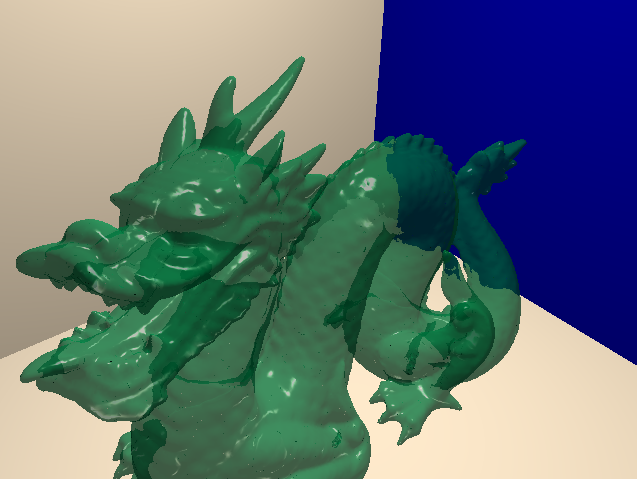
\includegraphics[width=7.2cm, height=5.4cm]{RefractionDragon}};
      \foreach \x in {-8,0,...,8} \draw[color=black] (\x,-6) -- (\x, 6);
      \foreach \y in {-6,-5.75,...,6} \draw[color=black] (-8,\y) -- (8, \y);
    \end{tikzpicture}
    \label{fig:sequentialRayWarp}
  }
  \hspace{20pt}
  \subfloat[Spatially coherent ray tracing. Fewer warps will now
    ray trace the dragon and the spatial coherence between rays
    results in entire warps raytracing the same side of the box.]{
    \begin{tikzpicture}[y=0.45cm, x=.45cm,font=\sffamily]
      \node {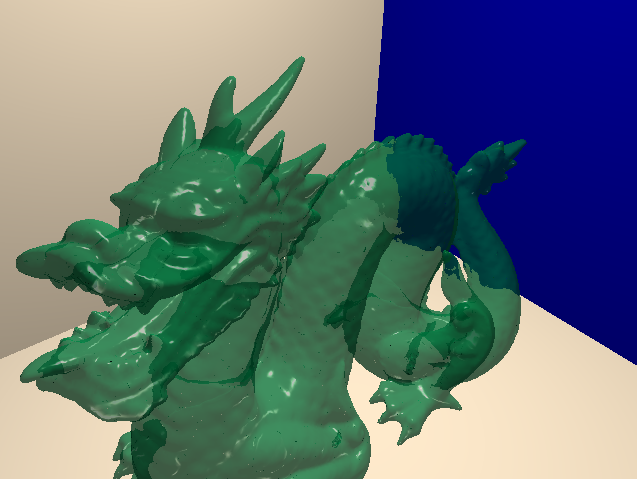
\includegraphics[width=7.2cm, height=5.4cm]{RefractionDragon}};
      \foreach \x in {-8,-7,...,8} \draw (\x,-6) -- (\x, 6);
      \foreach \y in {-6,-4,...,6} \draw (-8,\y) -- (8, \y);
    \end{tikzpicture}
    \label{fig:coherentRayWarp}
  }
  \caption[Sequantial and spatially coherent rays per warp.]{}
\end{figure}

The calculations needed to transform sequentially ordered ray ids into spatially
local ray ids are quite simple and can be seen in \refalg{alg:packet}. The
performance benefits gained by tracing spatially coherent rays and sharing
fetched global data among the rays in a warp are enormous, as seen in
\vreffig{fig:rayTracerEvaluation}.

It should be noted that a possibility exists that rays reflected multiple times
may eventually diverge completely and no longer be spatially coherent, but this
is no more of a problem for spatially local ray packets, than it is with the
sequential ray tracing approach and the spatially local ray packets will still
speed up primary rays.

\begin{algorithm}
  \caption{Converting a thread id to a ray id.}
  \label{alg:packet}
  \begin{algorithmic}
    \PROCEDURE{PacketID}
              {$thread$ : id}
              {$ray$ : id}
              {\COMMENTIT{Calculate the index of the packet cell.}
                \ASSIGN{$p_{id}$}{$thread / (p_{width} * p_{height})$}
                \COMMENTIT{Then compute the location of that cell in the grid of packets.}
                \ASSIGN{$grid_x$}{$p_{id} \mod  (image_{width} / p_{width})$}
                \ASSIGN{$grid_y$}{$p_{id} / (image_{width} / p_{width})$}
                \COMMENTIT{Compute the location of the ray inside that packet cell.}
                \ASSIGN{$p_x$}{$threads \mod  p_{width}$}
                \ASSIGN{$p_y$}{$(threads \mod (p_{width} * p_{height})) / p_{width}$}
                \COMMENTIT{Finally compute the location of the ray inside the grid and return the ray id.}
                \ASSIGN{$ray_x$}{$grid_x * p_{width} + p_x$}
                \ASSIGN{$ray_y$}{$grid_y * p_{height} + p_y$}
                \ASSIGN{$ray$}{$ray_x + ray_y * screen_{width}$}
              }
  \end{algorithmic}
\end{algorithm}


\subsection{Skipping Leaf Nodes}

% Inspired by Empty Space Maximization

The final ray tracer optimization presented in this thesis is inspired by the
early out option provided by Empty Space Maximization.

%% and combines the simple traversal of kd-trees with the bvh-tree's rigorous
%% intersection checks.

Since the only information available to rays traversing a kd-tree is the
position of the splitting plane and not the bounding volume of the node, the ray
can easily get sidetracked and end up in leaf nodes, whose bounding box it does
not even intersect. \Reffig{fig:waywardRay} is a simple example of
this. Extending the ray, $R(t) = t \vectwoT{1}{1} + \vectwoT{-4}{0}$, we can
clearly see that it will intersect leaf node 2. Unfortunately, when using
kd-trees, the only information available to the ray is that the node is split
along the y-axis at position 3, which in the above example causes the ray to get
sidetracked into leaf 1. This is a problem in scenes with large empty areas that
a ray has to traverse. Each time the ray intersects a splitting plane in those
empty areas, it can get sidetracked and traverse subtrees, whose associated
geometry the ray does not intersect.

%% An example of this is the great hall in the Sponza scene, where applying this
%% optimization will yield quite a performance increase, as can be seen in
%% \reffig{fig:rayTracerEvaluation}.

Empty Space Maximization has shown us that providing an early out option for
rays that would otherwise get sidetracked can increase performance
substantially. 
%and that also applies to this case. 
Since the leaf's bounding boxes are known from the tree creation phase, they can
be used to provide such an early out option and quickly skip leaf nodes that the
ray does not intersect. This saves a ray a lot of triangle intersection tests.

This optimization is only possible because I've stored the leafs bounding box
and will not be applicable in scenes where only a kd-tree is available. 

%% It does however show a major flaw in the kd-tree acceleration structure and a
%% more general solution to diverging rays will be presented under Future Work
%% in \refchapter{chp:future}.

\begin{figure}
  \centering
  \subfloat{
    \begin{tikzpicture}[y=0.5cm, x=.5cm]
      \drawNode{0,0}{6,0}{6,6}{0,6}      

      %Splits
      \draw (0,3) -- (6,3);
      
      % Leaf names
      \draw (3,1.5) node[leaf]{1};
      \draw (3,4.5) node[leaf]{2};

      \axes{7}{7}

      \drawRay{-4,0}{-3,1}
      \draw[line width=0.75pt, dashed, ->, color=gray] (-3,1) -- (0,4);
    \end{tikzpicture}
    \label{fig:waywardScene}
  }
  \subfloat{
    \begin{tikzpicture}[y=0.5cm, x=.5cm,font=\sffamily,
        level/.style={sibling distance=25mm/#1}]
      \node [visitedNode] (0){$y:3$}
        child {node [visitedLeaf] (1) {1}}
        child {node [leaf] (2) {2}}
        ;
    \end{tikzpicture}
    \label{fig:waywardTree}
  }
  \caption{A ray straying into a tree node, whose bounding box it does
    not intersect.}
  \label{fig:waywardRay}
\end{figure}

% Is not a general kd-tree optimization. Only works because we already
% have the bounding boxes from the tree creation phase and won't
% deallocate the space.




\section{Ray/Triangle Intersection}\label{sec:intersection}

The inherent diverging behaviour of rays traversing the kd-tree makes them hard
to parallize efficiently on the graphics card, since data access will be nearly
impossible to coalesce. The solution is to have enough active warps to
effectively hide the latency from global data fetching. This means that each
rays register usage must be kept to a minimum, in order to have enough memory
for as many active warps as possible.

Deciding which ray/triangle intersection method to use when ray tracing can
lower register usage and thus yield a significant performance boost.

% Consists of 2 parts. Ray/plane intersection which tells us the
% distance the ray will travel, and ray/triangle tests which tells us
% if the ray intersected the triangle.

Ray/triangle intersection can be broken down into two parts: A \textit{ray/plane
  intersection} test, which computes the signed distance, $t$, a ray must travel
to intersect the plane spanned by a triangle, and a \textit{triangle inclusion}
test, which checks if the intersection point is located inside the triangle. The
inclussion test is usually performed by calculating the intersection point's
\textit{barycentric coordinates} within the triangle.

Every point on a triangle, $T$, with vertices $T_a$, $T_b$ and $T_c$, can be described
as

\begin{displaymath}
  T(u,v) = (1-u-v)T_a + uT_b + vT_c, 0 \le u, 0 \le v, u+v \le 1
\end{displaymath}
 
where $(u, v)$ are the aforementioned barycentric coordinates. For a barycentric
coordinate to be inside $T$ it must therefore fulfill the requirements $0 \le
u$, $0 \le v$ and $u+v \le 1$.

Just as barycentric coordinates are used to linearly interpolate the vertex
positions across the triangle, they are also important for interpolating other
vertex attributes, such as normals or colors.

The following two ray/triangle intersection methods both compute the signed
distance and barycentric coordinates.

\subsection{Möller-Trumbore}

% One of the most popular intersection algorithms and featured in
% Real-Time Rendering.

The algorithm presented in Möller-Trumbore\citebook{MollerTrumbore97} is one of
the most popular algorithms for ray/triangle intersection, probably in no small
part due to its appearence in chapter 16.8 of Real-Time
Rendering\citebook{RTR3}, but also because it is one of the fastest ray/triangle
intersection algorithms that do not rely on extra memory or preprocessing of the
triangle before ray tracing.

% Calculates the transformation that transform the triangle into the
% unit triangle and applies this transformation to the ray.

Möller-Trumbore\citebook{MollerTrumbore97} exploits the fact that computing the
intersection between a triangle, $T(u, v)$ and ray, $R(t) = tR_{dir} + R_{ori}$ is
equivalent to solving the linear system of equations, the \textit{ray/triangle
  intersection equation}

%% The basic idea of the algorithm is to find the affine transformation
%% that, when applied to the triangle $T(u,v)$, transforms it into the unit
%% triangle, $U$, which has vertices $\vecthreeT{0}{0}{0}$,
%% $\vecthreeT{1}{0}{0}$ and $\vecthreeT{0}{1}{0}$. That affine
%% transformation is then applied to the ray, $R(t) = O + tD$, which
%% yields the vector $\vecthreeT{t}{u}{v}$, where $t$ is the distance to
%% the plane spanned by $T(u,v)$ and $u$ and $v$ are the barycentric
%% coordinates of the intersection point.

%% In short this boils down to solving the linear system of equations,
%% the \textit{ray/triangle intersection equation}

\begin{displaymath}
  \begin{array}{rl}
    & R(t) = T(u,v) \\
    \Updownarrow \\
    & tR_{dir} + R_{ori} = (1-u-v)T_a + uT_b + vT_c \\
  \end{array}
\end{displaymath}


Solving the ray/triangle intersection equation amounts to determining the signed
distance from the ray to the triangle, $t$, and the barycentric coordinates,
$(u, v)$. In \citebook{MollerTrumbore97} this is done by rearranging the terms
and applying Cramer's Rule, and the solution then becomes

\begin{displaymath}
  \vecthree{t}{u}{v} = \frac{1}{p \cdot e_1} 
  \vecthree{q \cdot e_2}{p \cdot r}{q \cdot R_{dir}}
\end{displaymath}

where $e_1 = T_b - T_a$, $e_2 = T_c - T_a$, $r = R_{ori} - T_a$, $p = R_{dir} \times  e_2$
and $q = r \times  e_1$.

\subsubsection{Implementation}

The implementation of this method is pretty straightforward using CUDA's vector
primitives and can be seen in \refalg{alg:moellerTrumbore}. The implementation
provided in \citebook{MollerTrumbore97} was optimized for the CPU and therefore
provided a lot of early out options as soon as the algorithm detected that a ray
had missed the triangle. Due to the synchonized behaviour of threads in the same
warp, providing as many early out possibilities as \citebook{MollerTrumbore97}
causes a branching overhead and results in reduced performance. This is
understandable since only one ray needs to intersect its triangle in order for
every thread in the warp to have to wait for it to finish. For the ray tracers
implemented as part of this thesis the optimal compromise was found to be only
providing one early exit after the ray/plane intersection and before computing
the barycentric coordinates.

\begin{algorithm}
  \caption{Möller-Trumbore ray/triangle intersection test}
  \label{alg:moellerTrumbore}
  \begin{algorithmic}
    \PROCEDURE{Möller-Trumbore}
              {$T$ : triangle, $R$ : ray}
              {$hit$ : bool, $t$ : distance, $(u,v)$ : barycentric coordinates}
              {\ASSIGN{$E_1$}{$T.b - T.a$}
                \ASSIGN{$E_2$}{$T.c - T.a$}
                \ASSIGN{$T$}{$R.O - T.a$}
                \ASSIGN{$P$}{$R.D - E_2$}
                \ASSIGN{$Q$}{$T - E_1$}
                \ASSIGN{$determinant$}{$P \cdot E_1$}
                \ASSIGN{$t$}{$(Q \cdot E_2) / determinant$}
                \COMMENTIT{Provide early out if the triangle is behind
                  the ray.}
                \IF{$0 < t$}
                  \ASSIGN{$u$}{$(P \cdot T) / determinant$}
                  \ASSIGN{$v$}{$(Q \cdot R.D) / determinant$}
                  \ASSIGN{$hit$}{$0 \le u$ \textbf{and} $0 \le v$
                    \textbf{and} $u+v \le 1$}
                \ELSE
                  \ASSIGN{$hit$}{$false$}
                \ENDIF
              }
  \end{algorithmic}
\end{algorithm}


\subsection{Woop}

% Why Woop is better

While Möller-Trumbore's ray/triangle intersection approach requires minimal
storage, in the sense that it takes as input the vertex positions already stored
in global memory, it does unfortunately require quite a lot of registers, since
it needs to both store the ray's parameters aswell as the determinant and the
matrix $\vecthreeT{q \cdot e_2}{p \cdot r}{q \cdot R_{dir}}$. The high register
usage can be remedied by performing precalulations per triangle as described in
Chapter 5 of Sven Woops diploma thesis\citebook{woop:04:diplom}. The trade-off
is a higher per triangle storage requirement for the scene's geometry.

% Also translates the ray using the unit triangle.

%% Woop observed that 

%% As was the case with the Möller-Trumbore approach, Woops approach also
%% transforms the general ray/triangle intersection problem into a
%% ray/unit triangle intersection problem, where the solution is
%% trivially calculated.

He observed that the triangle, $T$, can be transformed into the unit triangle

\begin{displaymath}
  U(u, v) = (1-u-v)\vecthreeT{0}{0}{0} + u\vecthreeT{1}{0}{0} + v\vecthreeT{0}{1}{0}
\end{displaymath}

by applying an affine transformation, consisting of a linear transformation
matrix, $M$, and a translation vector, $n$, on each of $T$'s vertices $T_a$,
$T_b$ and $T_c$.

\begin{displaymath}
  U_v = M T_v + n, v \in \{a, b, c\}
\end{displaymath}

The inverse affine transformation is the one that transforms the unit
triangle into $T$.

\begin{displaymath}
  T_v = M' U_v + n', v \in \{a, b, c\}, M' = M^{-1}, n' = -M^{-1}n
\end{displaymath}

Given that we already know $T$ and $U$, $M'$ and $n'$ can be
constructed as follows

\begin{displaymath}
  \begin{array}{l}
    M' = \left[ T_a - T_c, T_b - T_c, (T_a - T_c) \times (T_b - T_c)
      \right]\\
    n' = T_c
  \end{array}
\end{displaymath}

We can then derive $M$ and $n$ from $M'$ and $n'$. 

\begin{displaymath}
  M = (M')^{-1},
  n = - M n'
\end{displaymath}

This requires $M'$ to be invertable, which it always is for
\textit{non-degenerate triangles}\footnote{A degenerate triangles is
  a triangles that has collapsed into a line or a point.}.

%% Applying the affine transformation described by $m$ and $n$ to the
%% ray/triangle intersection equation we get

%% \begin{displaymath}
%%   \begin{array}{rl}
%%     & m R(t) + n = m T(u,v) + n\\
%%     \Updownarrow \\
%%     & m (O + tD) + n = m ((1-u-v)a + ub + vc) + n \\
%%     \Updownarrow \\
%%     & m (O + tD) + n = (1-u-v)U_a + u U_b + v U_c \\
%%   \end{array}
%% \end{displaymath}

Applying the affine transformation described by $M$ and $n$ to the ray, $M R(t)
+ n = R'(t) = R'_{ori} + tR'_{dir}$, it is transformed into the same space as
the unit triangle. Computing the distance, $t$, and barycentric coordinates,
$(u,v)$ then becomes trivial.

\begin{displaymath}
  \begin{array}{l}
    t = - R'_{dir,z} / R'_{ori,z} \\
    u = t R'_{dir,x} + R'_{ori,x} \\
    v = t R'_{dir,y} + R'_{ori,y}
  \end{array}
\end{displaymath}

Since each dimension in $R'$ can be computed independently, we get 

\begin{displaymath}
  \begin{array}{l}
    t = - (M_z \cdot R_{dir} + n_z) / (M_z \cdot R_{ori}) \\
    u = t (M_x \cdot R_{dir} + n_x) + M_x \cdot R_{ori} \\
    u = t (M_y \cdot R_{dir} + n_y) + M_y \cdot R_{ori} \\
  \end{array}
\end{displaymath}

where $M_i$ is the i'th row of $M$.

\subsubsection{Implementation}

The implementation is straightforward. $M$ and $n$ are computed and stored in 3
four component vectors as $w_i = \left[M_i, n_i \right]$ prior to ray
tracing. During ray/triangle intersection each vector $w_i$ can then be loaded
into register memory one vector at a time. In practice this saves three
registers compared with the Möller-Trumbore approach and can yield a sizeable
performance increase, as can be seen in \vreffig{fig:rayTracerEvaluation}.

% early out

As in the implementation of Möller-Trumbore, the Woop implementation also only
has one early out option, which is placed right after the distance calculation.

% The extra space used by the precalcultations can be mitigated if the vertices
% are no longer needed.

Finally, the extra memory required for storing the precalculated $m$ and $n$ can
be mitigated if the triangles vertex positions are replaced by $m$. This is only
possible however, if the vertices are not used elsewhere in the ray tracer.

